\section{Discussion of Design Space and Limitations}
%\section{Discussion: Design, Limitations, \& Future Work}

Torta carves out a new point in the design space of
tools for generating step-by-step records of app actions
(\fig{fig:design-space}).
%
In contrast to prior systems that operate within a single application,
Torta is designed to be as application-agnostic as possible so that it
can work across arbitrary desktop applications. This design decision
means \textbf{\emph{giving up granularity for generality}}: Torta cannot perform
fine-grained domain-specific tracking within any particular application, but
rather operates at the level of GUI windows, shell commands, system
calls, and filesystem mutations. One future way to bridge this gap is to
implement a plug-in system similar to Burrito's~\cite{GuoBurrito2012} where users write
application-specific tracers to hook into Torta.


On the spectrum of manual to automated running of steps, Torta lies
mostly at the manual end. Its primary goal is to generate mixed-media
tutorials for people to consume by manually following the steps and
customizing based on their needs. In contrast, fully-automated scripting
engines serve a different purpose than tutorials: Their goal is to
automate a set of repetitive actions, \emph{not} to show people how to
manually perform those actions with accompanying pedagogical context. In sum,
Torta's output should primarily be thought of as a \emph{rich form of
documentation} to help people figure out how to perform tasks for themselves,
not as a fully-automated script.


Torta is situated at a point in the design space \rev{that makes it
well-suited for a range of filesystem-modifying and
command-line-heavy} software tasks.
%
%, so they are well-suited for Torta.
%
Even though our original motivation was full-stack
web development, Torta is also useful for other complex software
development tasks involving more than simply an IDE. For instance,
game programming tutorials use an IDE, a 3D level editor, various
multimedia editors for assets, and project management tools all tied
together by command-line scripts. Low-level systems programming
tutorials involve a mix of command-line and GUI tools for introspection,
debugging, and performance profiling. Sysadmin (system administration)
and DevOps tutorials touch many corners of the operating system at once.
Data science tutorials combine multiple programming languages with
GUI-based data acquisition/wrangling tools. Finally, scientific
researchers hack up ad-hoc workflows that span multiple scripting
languages, scientific libraries, and legacy research
tools~\cite{GuoPhD2012}, so they can use Torta to generate documentation
that can help colleagues reproduce and build upon their computational
experiments.
%
\rev{However, Torta is less well-suited for information-foraging-heavy
computing tasks such as scholarly research and CSCW-types of
communication workflows, since those involve fewer filesystem
modifications and shell commands. For those kinds of tasks, Torta simply acts
like a screencast recorder with window-based segmentation.}


\begin{figure}
%\vspace{16em}

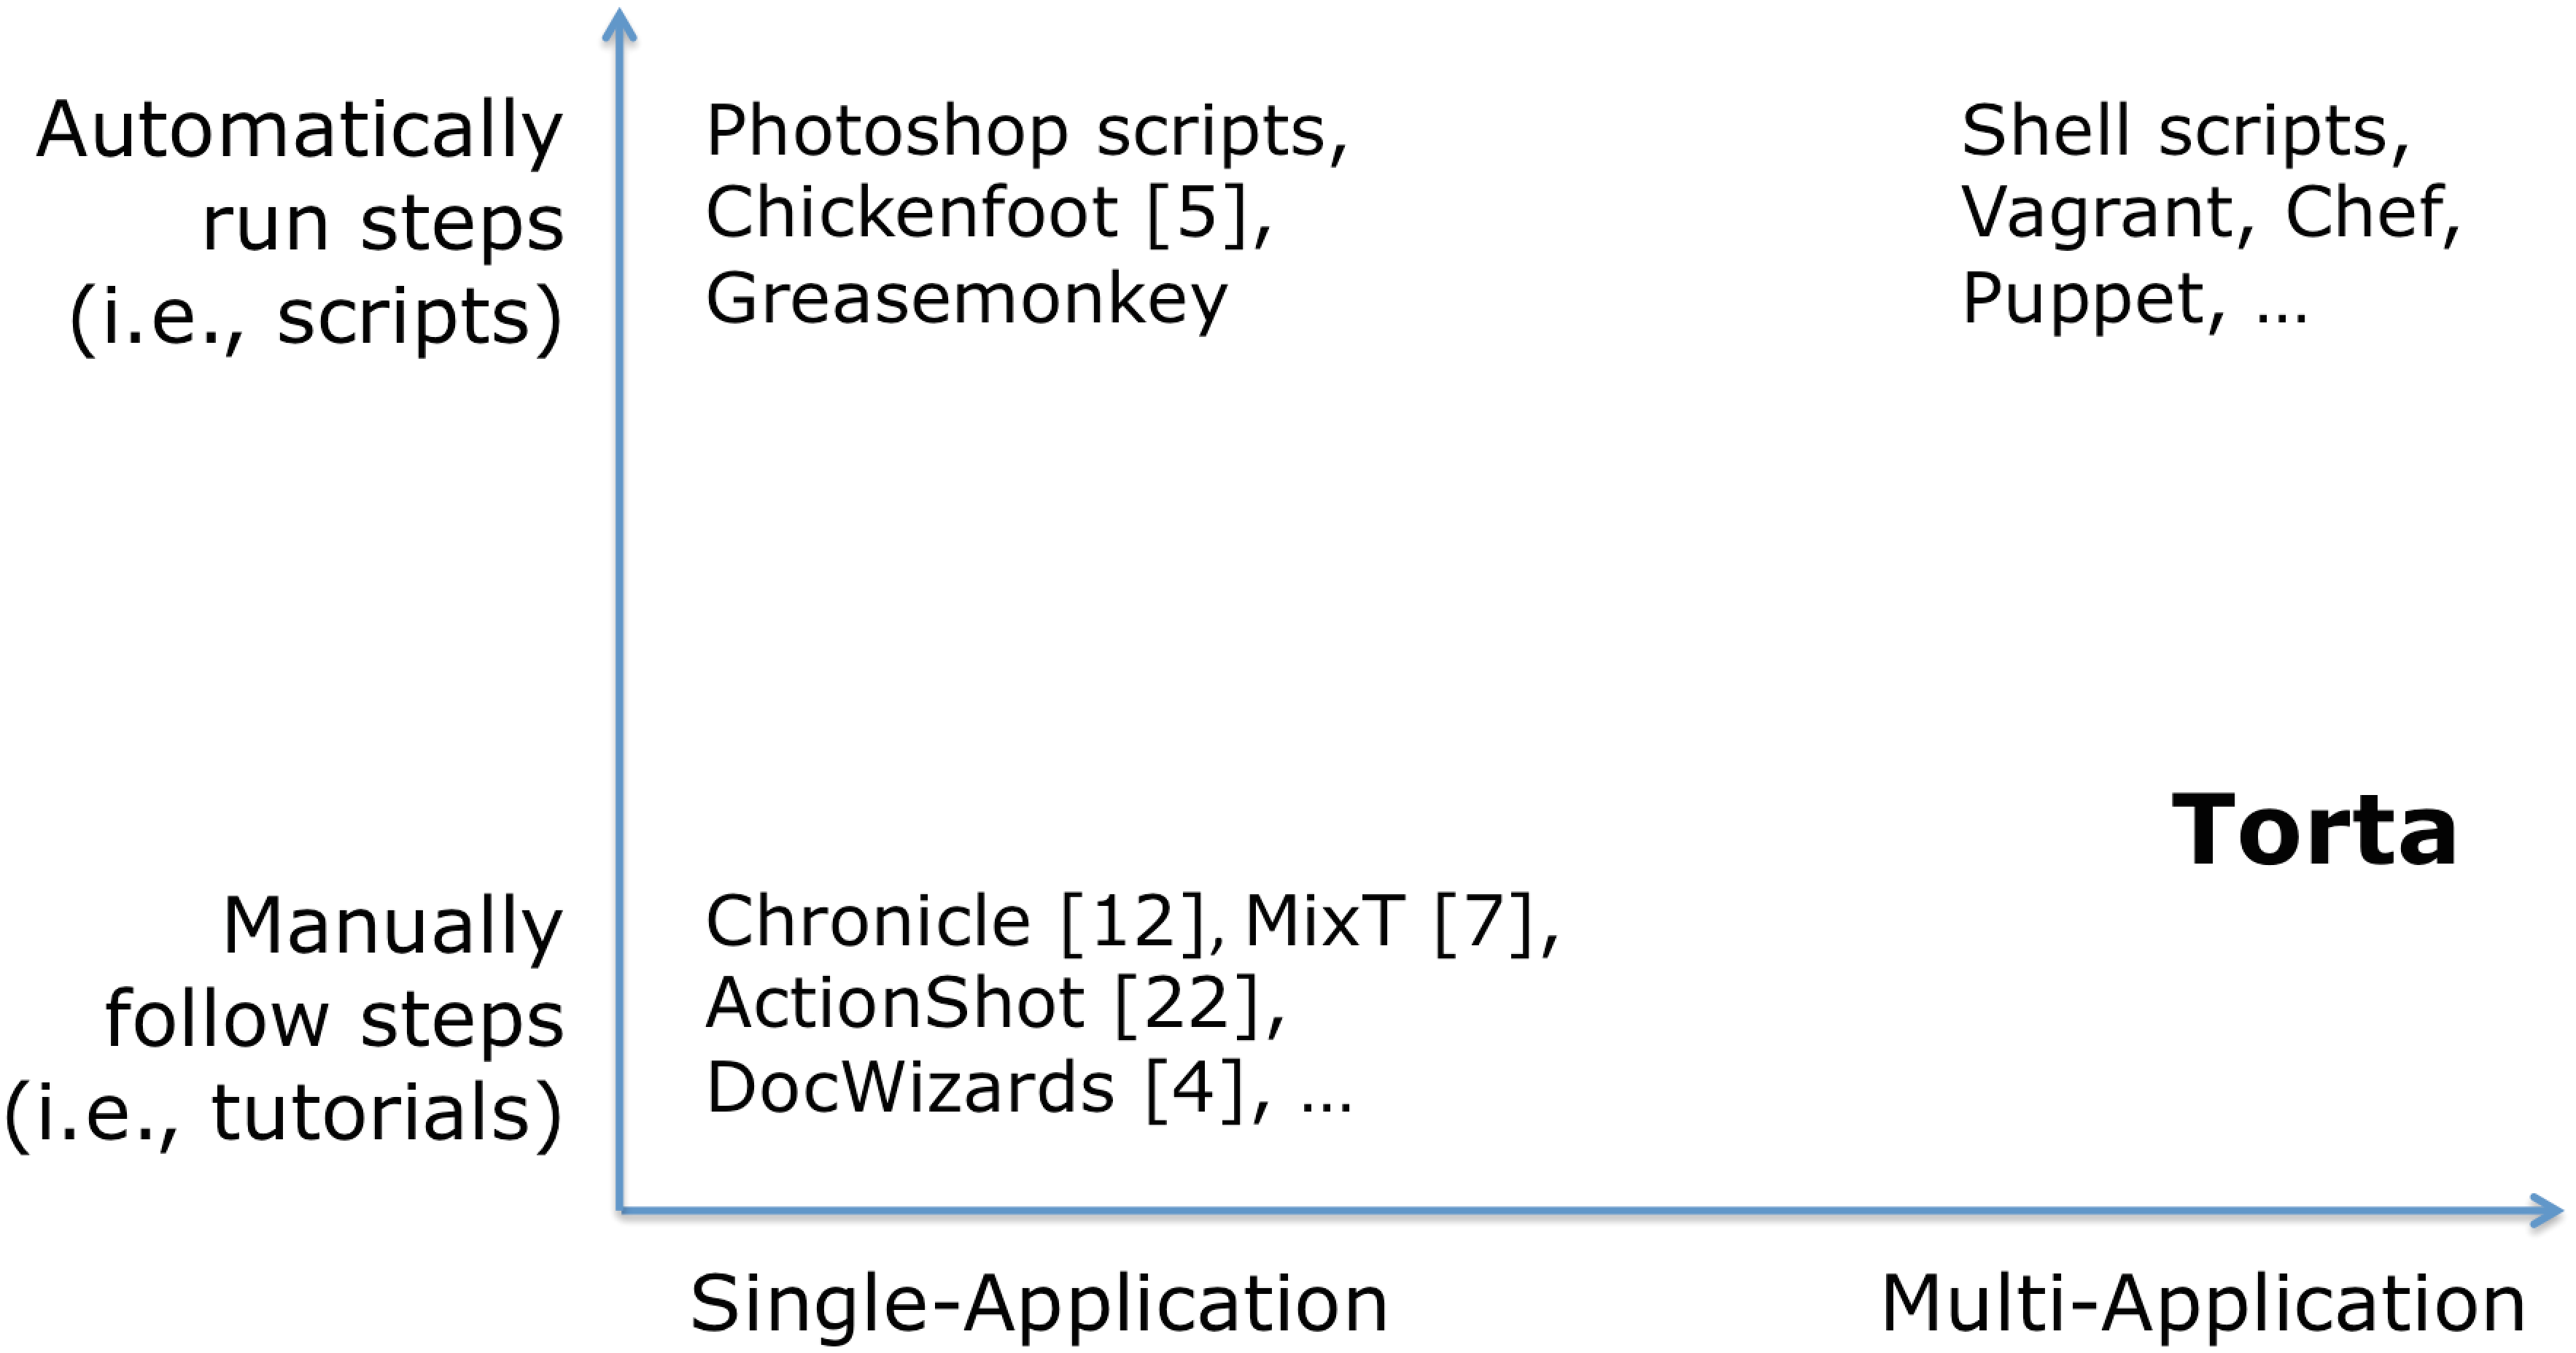
\includegraphics[width=\columnwidth]{figures/torta/design-space.png}

\nocite{Bolin2005} % cite Chickenfoot in the figure
\caption{The design space of tools for generating step-by-step records
of application actions, ranging from those that automatic run (i.e.,
scripts) to those meant for users to manually follow their steps (i.e.,
tutorials).}

\vspace{-0.5em} % stent
\label{fig:design-space}
\end{figure}


One of Torta's current limitations is that it supports recording and
editing only one user demonstration at a time. A future version of the
editor could support intelligent merging of multiple demonstrations
based on OS activity traces. Another limitation is that Torta does not
try to generalize the tutorial's contents: All recorded steps are
specific to the creator's single demonstration. Thus, it is up to the
creator to manually describe how each step could potentially be
generalized or customized by consumers. Again, a more intelligent editor
could take multiple demonstrations and semi-automatically infer possible
generalizations to make tutorials more robust.

Finally, even though automatically running certain steps can be
convenient, we have purposely not designed the Torta viewer as an
fully-automated tutorial runner. Differences between users' OS
setups and properties of specific applications make it impossible to
automatically run all steps with full accuracy.
Thus,
we still intend for users to manually follow tutorial steps and
only use automatic running as a supplement.


\section{Conclusion}

We presented Torta, an end-to-end system for recording, editing, and
consuming \rev{mixed-media tutorials that span multiple GUI and
command-line applications. The core technical insight that underpins
Torta is that the operating system already keeps track of vital
filesystem and process-level metadata necessary for segmenting tutorial
steps}. Thus, combining operating-system-wide activity tracing with
screencast video recording makes it possible to quickly create complex
GUI and command-line app tutorials by demonstration. \rev{Torta's
application-agnostic design} makes it well-suited for creating
tutorials in domains such as software development, data science, system
administration, and computational research.
%
\rev{We hope that it will inspire the design of future tutorial systems
that bridge the gap between video- and text-based formats.}

